\chapter{THE SMALL CURRENT ELEMENT: HERTZ DIPOLE}
Let us consider the simplest case of the current distribution which is a small current element of very finite elements $d\vec{l}$ whose direction is specified by the direction in which the current flows. This current distribution is the smallest current distribution possible and any other current distribution is the superposition of this small element. The choice of a small current element gives the foundation for finding electric and magnetic field for any arbitrary current distribution.

The small current element is also referred to as the \textbf{hertz dipole} which is characterized by what is called the current moment. The current moment is the product of the current and the length of the element, $Id\vec{l}$. For the current distribution we assume a sinusoidally varying time varying function for our analysis such that $I = I_od\vec{l}e^{j\omega t}$. This current element can be imagined as a small rod of cross sectional area which carries $\vec{J}$ such that the integral over the cross sectional area gives the current which multiplied by the length of the rod $d\vec{l}$ gives the current moment. Hence $\int_v\vec{J}dv' = I_od\vec{l}e^{j\omega t}$(with the assumption the assumption that the current is constant across the length of the rod $d\vec{l}$). 

Now, we will determine the vector potential $\vec{A}$ at some point in space given by $(r, \theta, \phi)$ in the spherical coordinate system, as shown in fig 3.1. Also to simplify the solution we will place our source(current element) at the origin.
\begin{figure}[h]
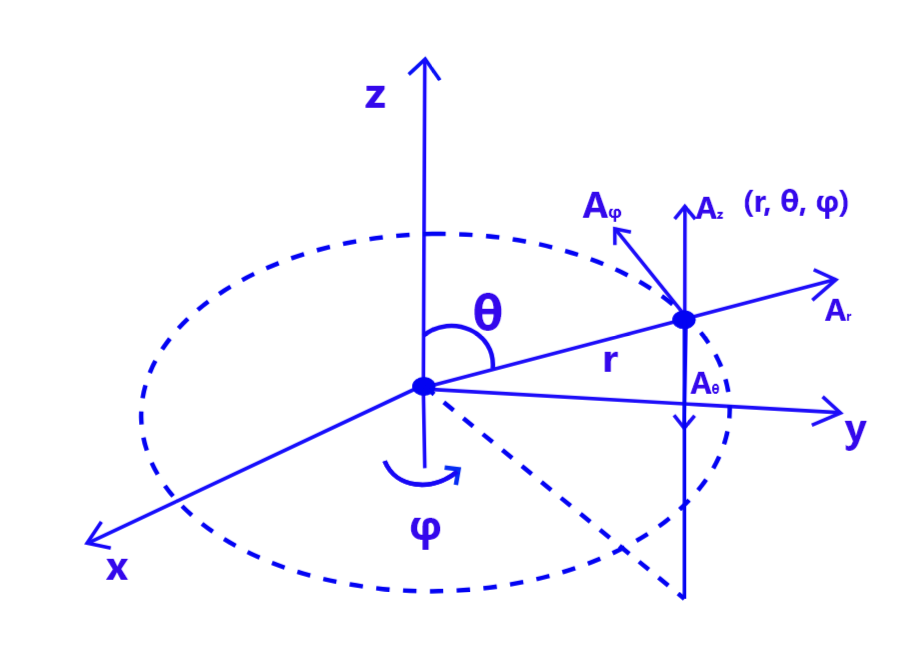
\includegraphics[width=1\linewidth]{./graphics/fig1_1}
\centering
\caption{}
\label{fig:1}
\end{figure}\newline
From the solution of the differential equation from previous lecture, recall that;
$$ \vec{A}(\vec{r}) =\int_v \dfrac{\mu \vec{J}(\vec{r'}) e^{-j\beta r}}{4\pi r}dv'$$ 
Notice r is substituted for $|\vec{r} - \vec{r'}|$ because $\vec{r'}$ is the position where the current element is located. Also since the length of the current element is much smaller compared to $r$, then $\dfrac{e^{-j\beta r}}{4 \pi r}$ is practically constant and 
$$ \vec{A}(\vec{r}) = \dfrac{\mu e^{-j\beta r}}{4 \pi r}\int_v\vec{J}(\vec{r'})dv'$$
$$  = \dfrac{\mu I d\vec{l} e^{-j\beta r}}{4\pi r}, \ recall \ I = I_oe^{j\omega t}$$
From the expression above it can be seen that the direction of the vector potential is determined by the direction of $d\vec{l}$ and $d\vec{l}$ is oriented in the $z$ direction. $\vec{A} = A_z\hat{z} = \dfrac{\mu I_o e^{j\omega t} dl e^{-j\beta r}}{4\pi r}\hat{z}$. But we want our analysis to be done in the spherical coordinate axes $(r, \theta, \phi)$. So we will convert from the $z$ direction to the $(r, \theta, \phi)$ direction. However, the $z$ direction has components in the $r$ and $\theta$ direction only because the $\phi$ direction is perpendicular to the $z$ direction. The component $A_{r}$ and $A_{\theta}$ are given as;
$$ A_{r} = A_z cos\theta; \ \
A_{\theta} = - A_z sin\theta; \ \
A_{\phi} = 0 $$
Now, with the vector potential that have been determined we would find out the magnetic field through the relationship $\mu \vec{H} = \nabla \times \vec{A}$ (since $\vec{B} = \nabla \times \vec{A}$ and $ \vec{B} = \mu \vec{H}$)
\begin{equation*}
\vec{H} = \frac{1}{\mu} \nabla \times \vec{A} = \dfrac{1}{r^2 sin\theta}
\begin{vmatrix}
\hat{r} & r\hat{\theta} & rsin\theta\hat{\phi} \\
\frac{\partial }{\partial r} &  \frac{\partial }{\partial \theta} &  \frac{\partial }{\partial \phi} \\
A_r & rA_{\theta} & rsin\theta A_{\phi}
\end{vmatrix}
\end{equation*}
For the analysis there is r and $\theta$ dependence because the vector $\vec{A}$ is a function of r and in the $\theta$ direction the source would not appear the same that is at $\theta = 0$, we see the top of the current element while when $\theta = \frac{\pi}{2}$ we see a line. But in the $\phi$ direction the source is symmetrical so there is no $\phi$ dependence 
Hence, 
\begin{dmath*}
\vec {H} = \dfrac{1}{\mu r^2 sin\theta} \begin{vmatrix}
\hat{r} & r\hat{\theta} & rsin\theta\hat{\phi} \\
\frac{\partial }{\partial r} &  \frac{\partial }{\partial \theta} &  0 \\
A_r & rA_{\theta} & 0
\end{vmatrix} = 0 \hat{r} - 0\hat{\theta} + \dfrac{rsin\theta}{\mu r^2 sin\theta}\hat{\phi}\left( \dfrac{\partial }{\partial r}(rA_{\theta}) - \dfrac{\partial }{\partial \theta} A_r\right)
\end{dmath*}

$$ = \dfrac{\hat{\phi}}{\mu r}\left(\dfrac{\partial}{\partial r}(r(-A_z sin\theta)) - \dfrac{\partial}{\partial \theta}(A_z cos\theta)\right)$$ 
Recall; $A_z(r)$ i.e. $A_z$ is a function of $r$
$$ = \dfrac{\hat{\phi}}{\mu r} \left(-sin\theta\left(r\dfrac{dA_z}{dr} + A_z\right) - A_z \dfrac{d(cos\theta)}{d\theta}\right)$$

$$ = -\dfrac{\hat{\phi}}{\mu r} (sin\theta\left(r\dfrac{dA_z}{dr} + A_z\right) - A_zsin\theta)$$

$$ = -\dfrac{sin\theta\hat{\phi}}{\mu r} \left(r\dfrac{dA_z}{dr} + A_z - A_z\right)$$

$$ = -\dfrac{sin\theta\hat{\phi}}{\mu } \dfrac{dA_z}{dr}$$ 
Recall that $A_z = \dfrac{\mu I_o e^{j\omega t} dl e^{-j\beta r}}{4\pi r}$

$$So, \ \dfrac{dA_z}{dr} = \dfrac{\mu I_o e^{j\omega t} dl}{4\pi}\dfrac{d}{dr}\left(\dfrac{e^{-j\beta r}}{r}\right)$$

$$ = \dfrac{\mu I_o e^{j\omega t} dl}{4\pi} \left(\dfrac{r(-j\beta e^{-j\beta r}) - e^{-j\beta r}}{r^2}\right)$$

$$ = \dfrac{\mu I_o e^{j\omega t}e^{-j\beta r} dl}{4\pi}  \left(\dfrac{-jr\beta - 1}{r^2}\right)$$

$$ = - \dfrac{\mu I_o e^{j\omega t}e^{-j\beta r} dl}{4\pi} \left(\dfrac{jr\beta}{r^2} + \dfrac{1}{r^2}\right)$$

$$ = - \dfrac{\mu I_o e^{(j\omega t-j\beta r)} dl}{4\pi} \left(\dfrac{j\beta}{r} + \dfrac{1}{r^2}\right)$$

\begin{equation}
\therefore \vec{H} = \dfrac{sin\theta I_o dl e^{j(\omega t-\beta r)} }{4\pi} \left(\dfrac{j\beta}{r} + \dfrac{1}{r^2}\right)\hat{\phi}
\end{equation}
With the magnetic field we apply maxwell's equation to find the electric field at a location in space where there is no charge or no source. So, we can substitute the magnetic field in the source free maxwell's equation given by $\nabla \times \vec{H} = j\omega \epsilon\vec{E}$ from the wave equations 
$$\vec{E} = \dfrac{1}{j\omega \epsilon}\nabla \times \vec{H};$$Also analyzing in  the spherical coordinate system, 
\begin{equation*}
\vec{E}  = \dfrac{1}{j\omega \epsilon} \times \dfrac{1}{r^2sin\theta}
\begin{vmatrix}
\hat{r} & r\hat{\theta} & rsin\theta\hat{\phi} \\ 
\dfrac{\partial}{\partial r} & \dfrac{\partial}{\partial \theta} &  \dfrac{\partial}{\partial \phi} \\
H_r & rH_\theta & rsin\theta H_\phi              
\end{vmatrix}
\end{equation*}
The magnetic field vector, $\vec{H}$ which we got has only the $\phi$ component. And the component is dependent on $r$ and $\theta$ only so the expression simplifies to 
\begin{equation*}
\vec{E}  = \dfrac{1}{j\omega \varepsilon} \times \dfrac{1}{r^2sin\theta}
\begin{vmatrix}
\hat{r} & r\hat{\theta} & rsin\theta\hat{\phi} \\ 
\dfrac{\partial}{\partial r} & \dfrac{\partial}{\partial \theta} &  0 \\
0 & 0 & rsin\theta H_\phi              
\end{vmatrix}
\end{equation*}
\begin{dmath*}
\vec{E}  = -\dfrac{j}{\omega \epsilon r^2sin\theta}
\begin{vmatrix}
\hat{r} & r\hat{\theta} & rsin\theta\hat{\phi} \\ 
\dfrac{\partial}{\partial r} & \dfrac{\partial}{\partial \theta} &  0 \\
0 & 0 & rsin\theta H_\phi              
\end{vmatrix}  = \dfrac{-j}{\omega  \epsilon r^2 sin\theta}\left(\hat{r} \dfrac{\partial}{\partial \theta}\left(rsin \theta H_{\phi}\right) - r\hat{\theta} \dfrac{\partial}{\partial r}(rsin\theta H_{\phi}) + 0\hat{\phi}\right)
\end{dmath*}

$$ = \dfrac{-j \hat{r}}{\omega \epsilon r^2 sin\theta}\dfrac{\partial}{\partial \theta}(rsin\theta H_{\phi}) + \dfrac{j \hat{\theta}}{\omega  \epsilon r sin\theta}\dfrac{\partial}{\partial r}(rsin\theta H_{\phi})$$ 

$$ = \dfrac{-j \hat{r}}{\omega  \epsilon r sin\theta}\dfrac{\partial}{\partial \theta}(sin\theta H_{\phi}) + \dfrac{j \hat{\theta}}{\omega  \epsilon r}\dfrac{\partial}{\partial r}(rsin\theta H_{\phi}) $$

$$ = \dfrac{-j \hat{r}}{\omega \epsilon r sin\theta}\left(sin\theta\dfrac{\partial }{\partial \theta}H_{\phi} + H_{\phi}\dfrac{d sin\theta}{d\theta}\right) + \dfrac{j\hat{\theta}}{\omega \epsilon r}\left(r\dfrac{\partial}{\partial r}H_{\phi} + H_{\phi}\right)$$
\smallskip
$$\vec{E} = E_r\hat{r} + E_{\theta}\hat{\theta}$$
\smallskip
$$E_r = \dfrac{-j \hat{r}}{\omega \epsilon r sin\theta}\left(sin\theta\dfrac{\partial }{\partial \theta}H_{\phi} + H_{\phi}\dfrac{d sin\theta}{d\theta}\right)$$

$$E_r = \dfrac{-j}{\omega \epsilon r}\dfrac{\partial}{\partial \theta}H_{\phi} - \dfrac{j cos\theta}{\omega \epsilon rsin\theta}H_\phi$$
\smallskip
Recall that $H_{\phi} = \dfrac{sin\theta I_o dl e^{j(\omega t-\beta r)} }{4\pi} \left(\dfrac{j\beta}{r} + \dfrac{1}{r^2}\right)$ from equation 3.1.
\smallskip
$$\dfrac{\partial H_{\phi}}{\partial \theta} =  \dfrac{I_o dl e^{j(\omega t-\beta r)} }{4\pi} (\dfrac{j\beta}{r} + \dfrac{1}{r^2})\dfrac{d (sin\theta)}{d \theta}$$

$$ = \dfrac{cos \theta I_o dl e^{j(\omega t-\beta r)} }{4\pi} \left(\dfrac{j\beta}{r} + \dfrac{1}{r^2}\right)$$
 
\begin{dmath*}
	E_r =  \dfrac{-j}{\omega \epsilon r}\left(\dfrac{cos \theta I_o dl e^{j(\omega t-\beta r)} }{4\pi} \left(\dfrac{j\beta}{r} + \dfrac{1}{r^2}\right)\right) -  \dfrac{j cos\theta}{\omega \epsilon rsin\theta}\dfrac{sin\theta I_o\vec{dl} e^{j(\omega t-\beta r)} }{4\pi} \left(\dfrac{j\beta}{r} + \dfrac{1}{r^2}\right)
\end{dmath*}

$$ = \dfrac{cos \theta I_o dl e^{j(\omega t-\beta r)} }{4\pi \omega  \epsilon} \left(\dfrac{\beta}{r^2} - \dfrac{j}{r^3}\right) + \dfrac{cos \theta I_o dl e^{j(\omega t-\beta r)} }{4\pi \omega \epsilon} \left(\dfrac{\beta}{r^2} - \dfrac{j}{r^3}\right) $$

$$ = \dfrac{2 cos \theta I_o dl e^{j(\omega t-\beta r)} }{4\pi \omega\epsilon} \left(\dfrac{\beta}{r^2} - \dfrac{j}{r^3}\right) $$
 
\begin{equation}
\therefore E_r = \dfrac{cos \theta I_o dl e^{j(\omega t-\beta r)} }{2\pi \omega \epsilon} \left(\dfrac{\beta}{r^2} - \dfrac{j}{r^3}\right)
\end{equation}
 
Also; 
$$ E_{\theta} = \dfrac{j}{\omega\epsilon r}\left(r\dfrac{\partial}{\partial r}H_{\phi} + H_{\phi}\right)$$ 

$$ =  \dfrac{j}{\omega \epsilon}\dfrac{\partial H_{\phi}}{\partial r} + \dfrac{j }{\omega \epsilon r}H_{\phi}$$

then,
\begin{dmath*}
\dfrac{\partial H_{\phi}}{\partial r} = \dfrac{sin \theta}{4 \pi} I_o dl \dfrac{d}{dr}\left(e^{j(\omega t - \beta r)}\left(\dfrac{j \beta}{r} + \dfrac{1}{r^2}\right)\right) = \dfrac{sin \theta}{4 \pi} I_o dl \left(e^{j(\omega t - \beta r)}\left(\dfrac{-j\beta}{r^2} - \dfrac{2}{r^3}\right) + (-j\beta)e^{j(\omega t - \beta r)}\left(\dfrac{j \beta}{r} + \dfrac{1}{r^2}\right)\right)
\end{dmath*}
$$ = \dfrac{sin \theta}{4 \pi} I_o dle^{j(\omega t - \beta r)} \left(\dfrac{-j\beta}{r^2} - \dfrac{2}{r^3} + \dfrac{\beta^2}{r} - \dfrac{j\beta}{r^2}\right)$$
$$ = \dfrac{sin \theta}{4 \pi} I_o dle^{j(\omega t - \beta r)} \left( \dfrac{\beta^2}{r} - \dfrac{2}{r^3}  - \dfrac{j2\beta}{r^2}\right)$$
So,
\begin{dmath*}
 E_{\theta} =  \dfrac{j}{\omega\epsilon}\dfrac{sin \theta}{4 \pi} I_o dle^{j(\omega t - \beta r)}\left( \dfrac{\beta^2}{r} - \dfrac{2}{r^3}  - \dfrac{j2\beta}{r^2}\right) + \dfrac{j}{\omega \epsilon r}\dfrac{sin\theta I_o\vec{dl} e^{(j\omega t-j\beta r)} }{4\pi} \left(\dfrac{j\beta}{r} + \dfrac{1}{r^2}\right)
\end{dmath*}
$$ = \dfrac{I_osin \theta dl e^{j(\omega t - \beta r)}}{4\pi \omega\epsilon}\left(\dfrac{j\beta^2}{r} - \dfrac{j2}{r^3} + \dfrac{2\beta}{r^2} - \dfrac{\beta}{r^2} + \dfrac{j}{r^3}\right)$$
\begin{equation}
\therefore E_{\theta} = \dfrac{I_osin \theta dl e^{j(\omega t - \beta r)}}{4\pi \epsilon}\left(\dfrac{j\beta^2}{\omega r} + \dfrac{\beta}{\omega r^2} - \dfrac{j}{\omega r^3}\right)
\end{equation}
Now we note that the magnetic field of the hertz dipole is oriented in the $\phi$ direction around $z$ axis while the electric field has two components: one in the $r$ direction which is the $r$ component and one in the $\theta$ direction which is the $\theta$ component .

A few important points emerge when studying the equations 3.1, 3.2 and 2.3, a careful look shows the expressions contains terms varying with $\frac{1}{r^3}$,$\frac{1}{r^2}$ and $\frac{1}{r}$. At points very close to the current element, the  $\frac{1}{r^3}$ term must be dominant. The variation of an electric field with  $\frac{1}{r^3}$ should remind us of electrostatic field of the dipole. The near field terms of  $\frac{1}{r^3}$ in the electric field component represent energy stored in a reactive(capacitive) field and they do not contribute to the radiated power. Also the  $\frac{1}{r^2}$ term in the $H_\phi$ expression is similarly important only in the region very near to the current element. It corresponds to the induction field of the dc current element as found through Biot-Savart law. 

At distance far away from the source, the effect of the  $\frac{1}{r^3}$ and  $\frac{1}{r^2}$ terms reduces drastically except for the effect of the  $\frac{1}{r}$ term, and we are said to be in the far-field zone. Thus the remaining fields that have the  $\frac{1}{r}$ dependence are the radiation fields. 

Let take look at equation (3.3), the term $\dfrac{\beta^2}{\omega r}$ can be further simplified to $\dfrac{\omega ^2\mu\epsilon}{\omega r} = \dfrac{\omega \mu \epsilon}{r}$, which means it varies inversely with r and is proportional to the frequency,$\omega$ . Also considering the $\dfrac{\beta}{\omega r^2}$ term, substituting $\beta = \omega \sqrt{\mu \epsilon}$ gives $\dfrac{\sqrt{\mu \epsilon}}{r^2}$ which is independent of the frequency, $\omega$ and the term $\dfrac{1}{\omega r^3}$ term (the electrostatic field), varies as $\dfrac{1}{\omega }$. \\ 
Hence at lower frequencies the $\dfrac{1}{\omega r^3}$ dominates while at higher frequencies the $\dfrac{\beta^2}{\omega r}$ dominates for the same current $I_odl$ which tallies with the statement established earlier that frequency increases the radiation increases. 

Lets better explain the electrostatic fields; it has been established that at lower frequencies this field dominates. For it to be called electrostatic field there must be charges but in our analysis we did not introduce charges, all we introduced was a current element where we assumed there is a current $I$ flowing through it. However, a new question is asked where does the current go? Current is the flow charges and we are considering time varying currents, so for half a cycle the flow of current is upward while on the second half the flow is downward. Considering the first half cycle the flow of current causes accumulation of positive charges at the top and negative charges at the bottom as shown in fig 3.2(a) below 
\begin{figure}[h]
\centering
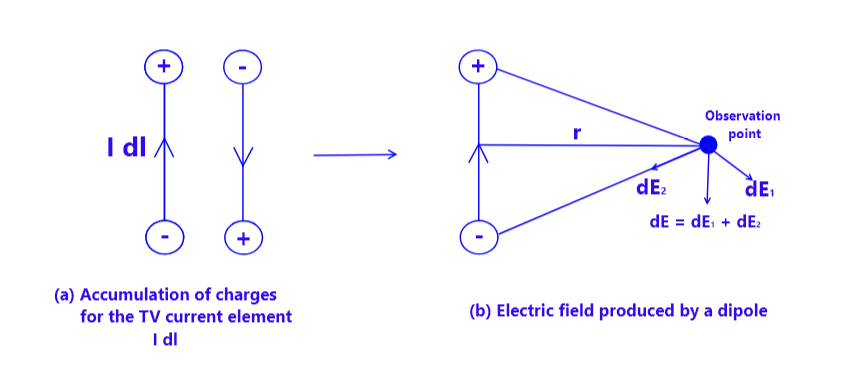
\includegraphics[width=0.7\linewidth]{./graphics/fig1_2}
\caption{}
\vspace{-20pt}
\label{fig:1}
\end{figure}
For the next half cycle the accumulation of positive charges occur at the bottom while the negative charges are accumulated at the top since the current is flowing downwards. So essentially, this current flow which is time varying is equivalent to having time varying charges that can be likened to an electric dipole whose charges are changing as a function of time. Considering a condition for a half cycle and calculating the electric field at an observation point a distance r from the dipole as shown in fig 3.2(b), gives an electric field which varies with $\frac{1}{r^3}$. Now the next question to ask is why does this field dominate at lower frequency? Well, we know that charge is the integral of current over time i.e. $Q =\int idt$, so for a time period which is very large for the same current amplitude the accumulated charges would be more. So as frequency goes on reducing the amount of charge that will get accumulated will increase. 

 Essentially, there are 3 fields; the electrostatic field, the induction field and the radiation field, which are generated by the simple Hertz dipole. Our interest however is the radiation field. 

From equation (3.3); Let $E_{\theta} = 0$

$$\Longrightarrow  \dfrac{j\beta^2}{\omega r} + \dfrac{\beta}{\omega r^2} - \dfrac{j}{\omega r^3} = 0 $$
\begin{center}
Taking the modulus
\end{center} 
$$  \dfrac{\beta^2}{\omega r} + \dfrac{\beta}{\omega r^2} - \dfrac{1}{\omega r^3} = 0 $$
\begin{center}
Multiply through by $\omega$
\end{center}
$$  \dfrac{\beta^2}{r} + \dfrac{\beta}{r^2} - \dfrac{1}{r^3} = 0 $$
\begin{center}
Multiply through by $r^3$
\end{center} 
$$  (r\beta)^2 + r\beta - 1 = 0 $$
$$  (r\beta)^2 + r\beta = 1 $$
$$  r\beta(r\beta + 1) = 1 $$
$$ r\beta = 1 \ or \ r\beta + 1 = 1 $$
$$ r = \dfrac{1}{\beta} \ or \ r = 0 $$
Since at $ r = 0$ the expression in equation (3.3) becomes undefined, then $ r = \dfrac{1}{\beta} $; $\beta = \dfrac{2\pi}{\lambda} \Longrightarrow r =  \dfrac{\lambda}{2 \pi} $ \\ 
At $ r =  \dfrac{\lambda}{2 \pi} $ the Electric field goes to zero and the plot is given in fig 3.3 below;
\begin{figure}[h]
\centering
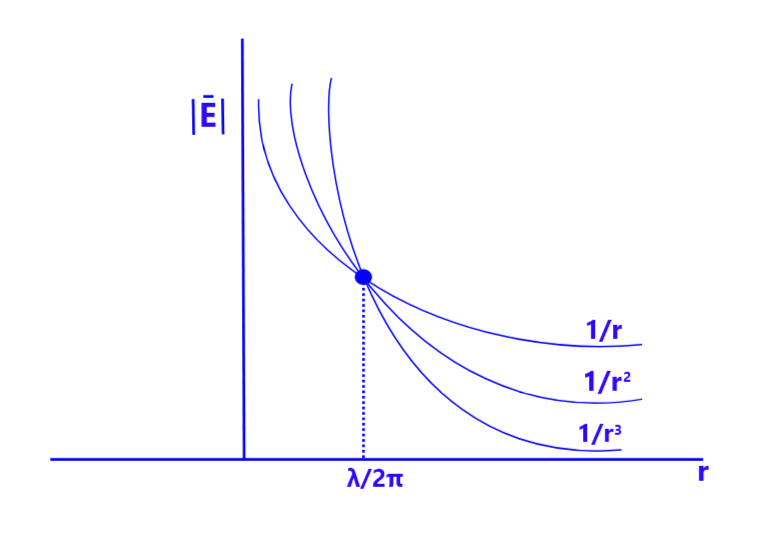
\includegraphics[width=1\linewidth]{./graphics/fig1_3}
\caption{}
\label{fig:1}
\end{figure}
Using the distance $r =  \dfrac{\lambda}{2 \pi}$ as the reference point and with this we will classify these fields into two categories;
\begin{enumerate}[(i)]
\item At $r \ll  \dfrac{\lambda}{2 \pi}$, we have the near Fields.
\item At $r \gg  \dfrac{\lambda}{2 \pi}$, we have the far Fields.
\end{enumerate}
The near fields consist of the three fields and as such consists of the $3$ components; $E_r$, $E_{\theta}$, and $H_{\phi}$. While the far field would consist of the radiation fields alone since every other field is negligible at the far field zone, so the far fields contains the $E_\theta$ and $H_\phi$ components only. 
$$E_{\theta} = j\dfrac{I_osin \theta dl\beta^2 e^{j(\omega t - \beta r)}}{4\pi \omega \epsilon r}$$
$$H_\phi = j\dfrac{I_o dl \beta \sin\theta   e^{(j\omega t-j\beta r)} }{4\pi r} $$

For the far-field which is our interest, we would note a few important points;
\begin{enumerate}
\item Both fields vary as a function $\theta$ (they both contain $sin\theta$) which implies as $\theta$ goes to zero the fields go to zero while they are maximum at $\theta = \dfrac{\pi}{2}$ which makes the field directional dependent. 
\item The ratio of $E_{\theta}$ and  $H_{\phi}$ gives the intrinsic impedance of the medium as shown below
$$\dfrac{E_{\theta}}{H_{\phi}} = \dfrac{\beta}{\omega  \epsilon} = \dfrac{\omega \sqrt{\mu \epsilon}}{\omega  \epsilon} = \sqrt{\dfrac{\mu}{\epsilon}} = \eta $$
\item Both components have the $j$ term which makes $90\deg$ out of phase with respect to $I_oe^{j\omega t}$. The reason is simple, recall that the radiation phenomenon is related to the rate of change of current, so for a time varying current which varies with $e^{j\omega t}$, the rate of change is equivalent to multiplying the quantity with $j\omega $ which result in fields with $90\deg$ phase difference to the current.
\item The wave we got is the spherical wave which is traveling in the $r$ direction and the $E_\theta$ and $H_\phi$ fields are oriented in the $\theta$ and $\phi$ direction respectively which means the fields and the direction of wave propagation are perpendicular to each other. This constitute essentially a Transverse Electromagnetic Wave, TEM, which is similar to the uniform plane wave.
\item Next, we concern ourselves with the polarization of the wave i.e. (in what way does the electric field vary as function of time?). We know the electric field is oriented in the $\theta$ direction which could be positive or negative as a function of time. This means the wave is linearly polarized.
\end{enumerate}